\documentclass{beamer}
\usepackage{fontspec} 
\usepackage{listings}
\usepackage[utf8]{inputenc}
\usepackage{fontspec}
\usepackage{minted}
\setsansfont{Calibri}
\setmonofont{Consolas}
\usetheme{CambridgeUS}
\title[Scalaz]{Scalaz\\Learn You Yet Another Real World Gentle Haskell (LYYARWGH) ((c) sproingie)}
\author{George Leontiev}
\institute{deltamethod GmbH}
\date{April 17, 2013}

\begin{document}

\begin{frame}
\titlepage
\centerline{($\lambda$x.folonexlambda-calcul.us)@}
\centerline{folone.info}
\end{frame}

\begin{frame}{Agenda}
  \begin{itemize}
    \item Some hotness without context, to draw attention (Option, Boolean, Memo)
    \item Typeclasses
    \item Monoid
    \item Functor, Applicative, Monad
    \item Effects
    \item scalaz 6 vs seven
    \item typelevel.org
  \end{itemize}
\end{frame}

\begin{frame}{What is scalaz}
  \begin{itemize}
    \item Purely functional datatypes (Fingertree, HList, DList, Trees, Zippers, Nel, ImmutableArray)
    \item Typeclasses
    \item Effects
    \item Concurrency
  \end{itemize}
\end{frame}

\begin{frame}[fragile]{Examples -- typesafe equals}
  \begin{minted}[mathescape,
               numbersep=5pt,
               gobble=2,
               framesep=2mm]{scala}
  s> "" == 5
  res0: Boolean = false

  s> "" === 5
  <console>:14: error: type mismatch;
   found   : Int(5)
   required: java.lang.String
             "" === 5
                    ^
  \end{minted}
  <spoiler>$\forall$ stuff $\in$ scalaz $\equiv$ scala.stdlib | stuff is typesafe $\vee$ stuff is strict</spoiler>\newline
  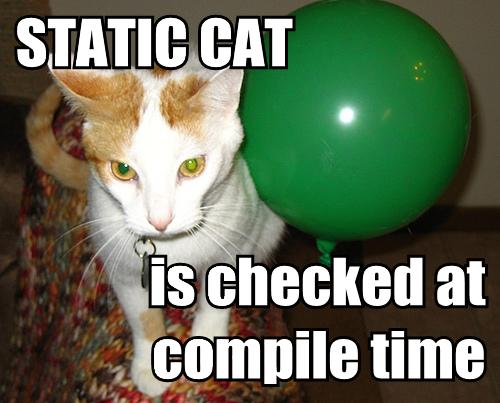
\includegraphics[scale=0.15]{static_cat}
\end{frame}

\begin{frame}[fragile]{Examples -- options}
  \begin{minted}[mathescape,
               numbersep=5pt,
               gobble=2,
               framesep=2mm]{scala}
  s> some(5) getOrElse 0
  res1: Int = 5
  s> some(5) | 0
  res2: Int = 5
  s> some(1) getOrElse "ok"
  res3: Any = 1
  s> some(1) | "ok"
  <console>:14: error: type mismatch;
   found   : java.lang.String("ok")
   required: Int
            some(1) | "ok"
                      ^
  s> ~some(5) // Monoids
  res4: Int = 5
  s> ~none[Int] // NB: Beware of unary_~ on Validations
  res5: Int = 0
  \end{minted}
\end{frame}

\begin{frame}[fragile]{Examples -- options II}
  \begin{minted}[mathescape,
               numbersep=5pt,
               gobble=2,
               framesep=2mm]{scala}
  // Smart constructors
  s> :t Some(1)        s> :t None
  Some[Int]            None.type
  s> :t some(1)        s> :t none[Int]
  Option[Int]          Option[Int]

  s> List(Some(1),None).foldLeft(None){(_, v) => v}
  <console>:14: error: type mismatch;
   found   : v.type (with underlying type Option[Int])
   required: None.type
     List(Some(1),None).foldLeft(None){(_, v) => v}
                                                 ^
  s> List(Some(1),None).foldLeft(none[Int]){(_, v) => v}
  res11: Option[Int] = None
  \end{minted}
\end{frame}

\begin{frame}[fragile]{Examples -- booleans}
  \begin{minted}[mathescape,
               numbersep=5pt,
               gobble=2,
               framesep=2mm]{scala}
  scala> true ? println("true") | println("false")
  true

  scala> true ?? 5        scala> true !? 5
  res14: Int = 5          res15: Int = 0

  scala> false ?? 5       scala> false !? 5
  res15: Int = 0          res17: Int = 5
  \end{minted}
\end{frame}

\begin{frame}[fragile]{Examples -- function composition}
  \begin{minted}[mathescape,
               numbersep=5pt,
               gobble=2,
               framesep=2mm]{scala}
  val a = (_:Int) + 6
  val b = (_:Int).toString
  val c = (_:String).length

  scala> 5 |> a |> b |> c
  res18: Int = 2

  scala> //(c $\cdot$ b $\cdot$ a) apply 5 // contramap
  res19: Int = 2

  scala> 5 |> //(a $\circ$ b $\circ$ c) // map
  res20: Int = 2

  // contramap === flip . map
  \end{minted}
\end{frame}

\begin{frame}[fragile]{Examples -- Memo}
  \begin{minted}[mathescape,
               numbersep=5pt,
               gobble=2,
               framesep=2mm]{scala}
  def func(s: String) = // Expensive computation
  scala> Memo.immutableHashMapMemo(func)
  res11: String => java.lang.String = <function1>

  // Different strategies
  mutableHashMapMemo
  arrayMemo // sized
  immutableListMemo
  immutableTreeMapMemo
  doubleArrayMemo // memoizing Double results != sentinel
  weakHashMapMemo // GC
  \end{minted}
\end{frame}

\begin{frame}[fragile]{Examples -- Trampoline}
  
\includegraphics[scale=0.2]{tailrec}
  \begin{minted}[mathescape,
               numbersep=5pt,
               gobble=2,
               framesep=2mm]{scala}
    def even(n: Int): Boolean =
      if (n == 0) true
      else odd(n - 1)
    def odd(n: Int): Boolean =
      if (n == 0) false
      else even(n - 1)

    scala> even(30000)
  \end{minted}
\end{frame}

\begin{frame}[fragile]{Examples -- Trampoline}
  
\includegraphics[scale=0.2]{tailrec2}
  \begin{minted}[mathescape,
               numbersep=5pt,
               gobble=2,
               framesep=2mm]{scala}
    def even(n: Int): Trampoline[Boolean] =
      if (n == 0) done(true)
      else suspend(odd(n - 1))
    def odd(n: Int): Trampoline[Boolean] =
      if (n == 0) done(false)
      else suspend(even(n - 1))

    scala> even(30000).run
  \end{minted}
\end{frame}

\begin{frame}[fragile]{Examples -- Trampoline}
  \begin{minted}[mathescape,
               numbersep=5pt,
               gobble=2,
               framesep=2mm]{scala}
  def fibRec(n: Int): Int =
    if (n < 2) n else fibRec(n - 1) + fibRec(n - 2)

  def fibTailrec(n: Int) = {
    def loop(n: Int, next: Int, result: Int) = n match {
      case 0 => result
      case _ => loop(n - 1, next + result, next)
    }
    loop(n, 1, 0)
  }
  \end{minted}
\end{frame}

\begin{frame}[fragile]{Examples -- Trampoline}
  \begin{minted}[mathescape,
               numbersep=5pt,
               gobble=2,
               framesep=2mm]{scala}
  def fibTramp(n: Int): Trampoline[Int] =
    if (n < 2) done(n) else suspend {
      for {
        i <- fibTramp(n - 1)
        j <- fibTramp(n - 2)
      } yield i + j
    }
  // Continuation monad magic
  \end{minted}
  
\includegraphics[scale=0.2]{cont}\newline
  Consult @runarorama's paper "Stackless Scala with Free Monads"
\end{frame}

\begin{frame}[fragile]{Typeclasses}
  \begin{center}
    
\includegraphics[scale=0.3]{monad_tutorial}\newline
    {\large \url{http://www.haskell.org/haskellwiki/Typeclassopedia} }
    {\large \url{http://typeclassopedia.bitbucket.org/} }
  \end{center}
\end{frame}

\begin{frame}[fragile]{Monoids}
\begin{center}
$(S, \otimes, 1)$\newline
$\forall a, b \in S: a \otimes b \in S$\newline
$\forall a, b, c \in S: (a \otimes b) \otimes c = a \otimes (b \otimes c)$\newline
$\forall a \in S: 1 \otimes a = a \otimes 1 = a$\newline
\end{center}
  \begin{minted}[mathescape,
               numbersep=5pt,
               gobble=2,
               framesep=2mm]{scala}
  trait Semigroup[F] {
    def append(a1: F, a2: F): F
  }
  trait Monoid[F] extends Semigroup[F] {
    def zero: F
  }
  // scalacheck-binding
  import scalaz.scalacheck.ScalazProperties._
  semigroup.laws[Int]
  monoid.laws[String]
  \end{minted}
\end{frame}

\begin{frame}[fragile]{Monoids}
  \begin{minted}[mathescape,
      numbersep=5pt,
      gobble=2,
      framesep=2mm]{scala}
    scala> 1 |+| 5
    res2: Int = 6

    scala> Multiplication(2) |+| Multiplication(3)
    res4: Int @@ Multiplication = 6

    scala> some(1) |+| some(5)
    res5: Option[Int] = Some(6)

    // Monoids beget monoids
    scala> some(some((1, "OH ", 1 + (_:Int)))) |+|
           some(some((4, "HAI", 2 * (_:Int))))
    res6: Option[Option[(Int, java.lang.String,
          Int => Int)]] = Some(Some((5, OH HAI,
                               <function1>)))
  \end{minted}
\end{frame}

\begin{frame}[fragile]{Monoids}
  \begin{minted}[mathescape,
      numbersep=5pt,
      gobble=2,
      framesep=2mm]{scala}
    scala> List(1,2,3).suml
    res16: Int = 6

    scala> List("OH ", "HAI", "!").suml
    res17: java.lang.String = OH HAI!
  \end{minted}
\end{frame}


\begin{frame}[fragile]{Functors}
  
\includegraphics[scale=0.5]{fmapfmapfmap}
  \begin{minted}[mathescape,
      numbersep=5pt,
      gobble=2,
      framesep=2mm]{scala}
    trait Functor[F[_]] {
      def fmap[A, B](f: A => B): F[A] => F[B]
    }

    scala> some(3) map(_.toString)
    res13: Option[java.lang.String] = Some(3)
  \end{minted}
\end{frame}

\begin{frame}[fragile]{Applicatives}
    \begin{minted}[mathescape,
      numbersep=5pt,
      gobble=2,
      framesep=2mm]{scala}
    trait Applicative[T[_]] extends Functor[T] {
      def pure[A](a: A): T[A]
      def <*>[A, B](tf: T[A => B])(ta: T[A]): T[B]
    }

    scala> some(1) <*> some((_:Int) + 2) <*> some((_:Int) * 5)
    res10: Option[Int] = Some(15)

    scala> List(1,2) <*> List((_:Int) * 5, (_: Int) + 2)
    res12: List[Int] = List(5, 10, 3, 4)
  \end{minted}
\end{frame}

\begin{frame}[fragile]{Applicatives}
    \begin{minted}[mathescape,
      numbersep=5pt,
      gobble=2,
      framesep=2mm]{scala}
      scala> List(some(1), some(2), some(3))
      res21: List[Option[Int]] = List(Some(1), Some(2),
                                      Some(3))

      scala> .sequence
      res22: Option[List[Int]] = Some(List(1, 2, 3))

      scala> res21.traverse(x => some(x))
      res23: Option[List[Int]] = Some(List(1, 2, 3))
  \end{minted}
\end{frame}

\begin{frame}[fragile]{Monads}
  \begin{minted}[mathescape,
      numbersep=5pt,
      gobble=2,
      framesep=2mm]{scala}
    trait Monad[M[_]] extends Applicative[M]{
      def >>=[A, B](ma: M[A])(f: A => M[B]): M[B]
    }

    scala> for {
     | i <- List(1,2,3)
     | j <- List(4,5,6)
     | } yield i*j
    res15: List[Int] = List(4, 5, 6, 8, 10, 12, 12, 15, 18)
  \end{minted}
\end{frame}

\begin{frame}[fragile]{IO}
  \begin{center}
    {\Huge DEMO }\newline
    \includegraphics[scale=0.4]{IO}
  \end{center}
\end{frame}

\begin{frame}{That's it}
  
\includegraphics[scale=0.4]{escape}\newline
  \Huge \centerline{Questions?}
\end{frame}

\end{document}
